
% This LaTeX was auto-generated from MATLAB code.
% To make changes, update the MATLAB code and republish this document.

\documentclass{article}
\usepackage{graphicx}
\usepackage{color}

\sloppy
\definecolor{lightgray}{gray}{0.5}
\setlength{\parindent}{0pt}

\begin{document}

    
    \begin{verbatim}
format long

InitialStep=1;
Eigenvalues=zeros(5,1);

NoVals=1;
Counter=1;
InitialSign=sign(g(InitialStep));

while NoVals<6
    x=Counter*InitialStep;
    if sign(g(x))~=InitialSign
        Eigenvalues(NoVals,1)=x;
        NoVals=NoVals+1;
        InitialSign=sign(g(x));
        disp('This clarifies that -1<g(p)<1 when h=0.1 is used')
        gError(x)
        disp("This calculates when |g'(p)| is smallest")
        gError(x)-gError(x-1)
    end
    Counter=Counter+1;
end

NoVals=1;
epsilon=abs(g(Eigenvalues(4,1))-g(Eigenvalues(4,1)-1))*5*10^(-6)

while NoVals<6
    LowerP=Eigenvalues(NoVals,1)-1;
    UpperP=Eigenvalues(NoVals,1);
    if g(LowerP)==g(UpperP)
        error('The g value must differ at these bounds')
    end

    if g(LowerP)<g(UpperP)
        gradient=+1;
    else
        gradient=-1;
    end

    while true
        P=(g(UpperP)*LowerP-g(LowerP)*UpperP)/(g(UpperP)-g(LowerP));
        if abs(g(P))<epsilon
            break
        else
            %This checks what the gradient is at the root
            if g(LowerP)<g(UpperP)
                gradient=+1;
            else
                gradient=-1;
            end
            %This determines which bound should be replaced
            if g(P)*gradient<0
                LowerP=P;
            else
                UpperP=P;
            end
        end
    end
    Eigenvalues(NoVals,1)=P;
    NoVals=NoVals+1;
end
disp('Eigenvalues:')
disp(Eigenvalues)
digits(16)
latex(sym(vpa(Eigenvalues)))

NoVals=1;
while NoVals<6
    m=RK4Vector(0,1,0,1,0.001,Eigenvalues(NoVals),8);
    A=trapz(m(:,2).^2./((1+m(:,1)).^(8)))*Eigenvalues(NoVals)^2;
    m(:,2)=(1/sqrt(A)).*m(:,2);
    figure
    plot(m(:,1),m(:,2))
    xlabel('x')
    ylabel('y')
    print(strcat('Image_9_',num2str(NoVals)),'-depsc')
    NoVals=NoVals+1;
end

function answer=gError(x)
    answer=RK4Vector(0,1,0,1,0.1,x,8);
    answer=answer(end,2);
end

function answer=g(x)
    answer=RK4Vector(0,1,0,1,0.001,x,8);
    answer=answer(end,2);
end

function Solution = RK4Vector(x_0,x_n,y_0,z_0,h,p,a)
%Creates the table of iterates
X=zeros(ceil(x_n/h)+1,1);
Y=zeros(ceil(x_n/h)+1,2);
Y(1,:)=[y_0,z_0];
X(1)=x_0;
counter=2;

%This fills the table using the runge kutta method
while counter<=ceil((x_n-x_0)/h)+1
    X(counter)=(counter-1)*h;
    K1=h*F(X(counter-1),Y(counter-1,:),p,a);
    K2=h*F(X(counter-1)+h*1/2,Y(counter-1,:)+K1/2,p,a);
    K3=h*F(X(counter-1)+h*1/2,Y(counter-1,:)+K2/2,p,a);
    K4=h*F(X(counter-1)+h,Y(counter-1,:)+K3,p,a);
    Y(counter,:)=Y(counter-1,:)+(K1+2*K2+2*K3+K4)/6;
    counter=counter+1;
end
Solution=[X,Y];
end

%This is f(X,Y)
function out = F(x,Y,p,a)
    out=zeros(1,2);
    %f_1
    out(1)=Y(2);
    %f_2
    out(2)=-p^2*(1+x)^(-a)*Y(1);
end
\end{verbatim}

        \color{lightgray} \begin{verbatim}This clarifies that -1<g(p)<1 when h=0.1 is used

ans =

  -0.060822965514468

This calculates when |g'(p)| is smallest

ans =

  -0.097950909801548

This clarifies that -1<g(p)<1 when h=0.1 is used

ans =

   0.038738798160780

This calculates when |g'(p)| is smallest

ans =

   0.045795354206171

This clarifies that -1<g(p)<1 when h=0.1 is used

ans =

  -0.099774421005125

This calculates when |g'(p)| is smallest

ans =

  -0.022385780959368

This clarifies that -1<g(p)<1 when h=0.1 is used

ans =

   0.056336230888559

This calculates when |g'(p)| is smallest

ans =

  -0.014001439055975

This clarifies that -1<g(p)<1 when h=0.1 is used

ans =

  -0.688656876900669

This calculates when |g'(p)| is smallest

ans =

   0.097498275834061


epsilon =

     1.347968275757026e-07

Eigenvalues:
  10.358921780539527
  21.263930772860803
  32.105385390751429
  42.919336546690445
  53.719111878919733


ans =

    '\left(\begin{array}{c} 10.35892178053953\\ 21.2639307728608\\ 32.10538539075143\\ 42.91933654669045\\ 53.71911187891973 \end{array}\right)'

\end{verbatim} \color{black}
    
\includegraphics [width=4in]{Question_9_1_01.eps}

\includegraphics [width=4in]{Question_9_1_02.eps}

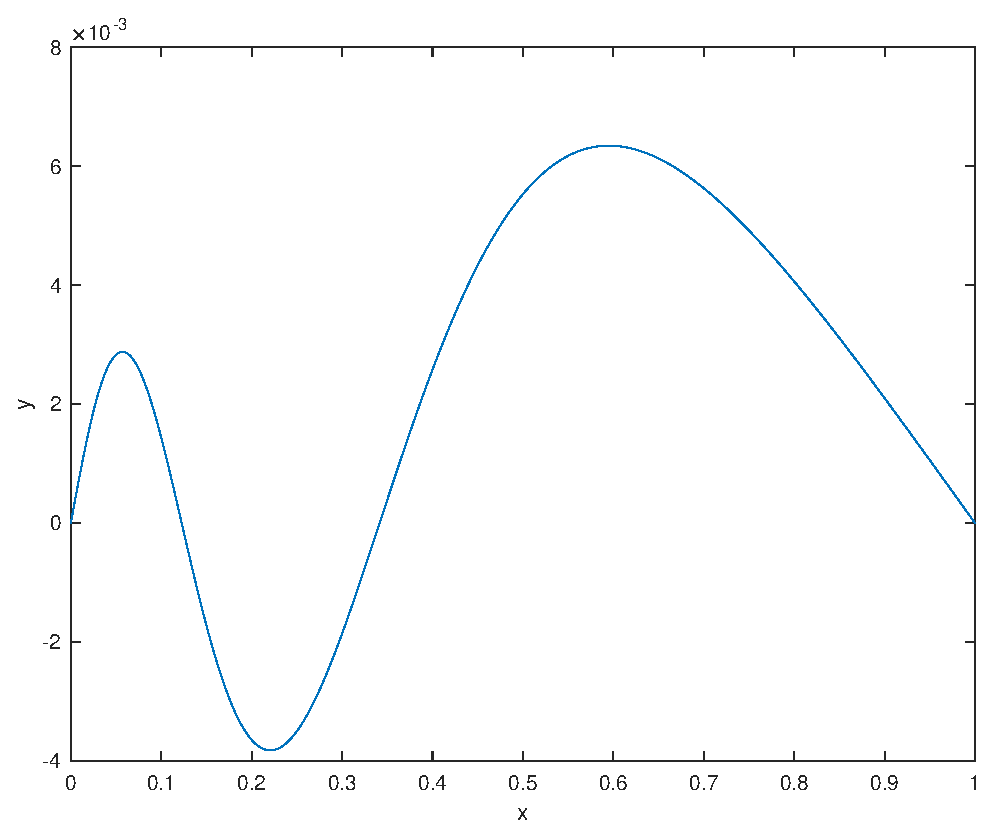
\includegraphics [width=4in]{Question_9_1_03.eps}

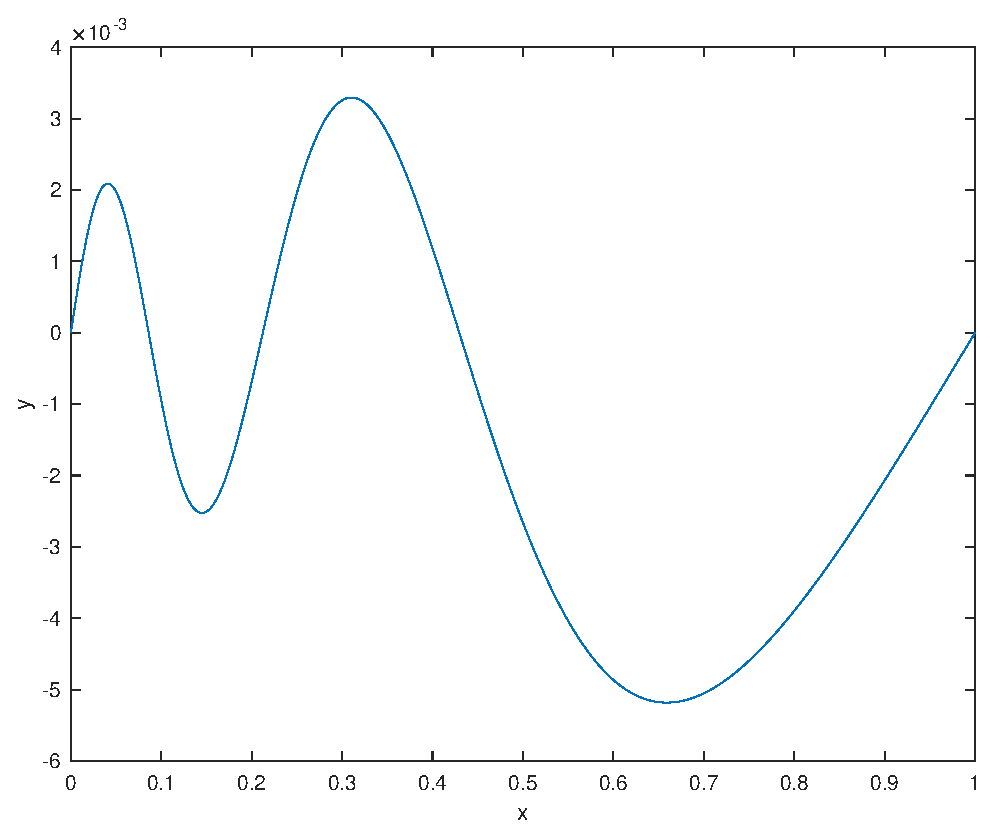
\includegraphics [width=4in]{Question_9_1_04.eps}

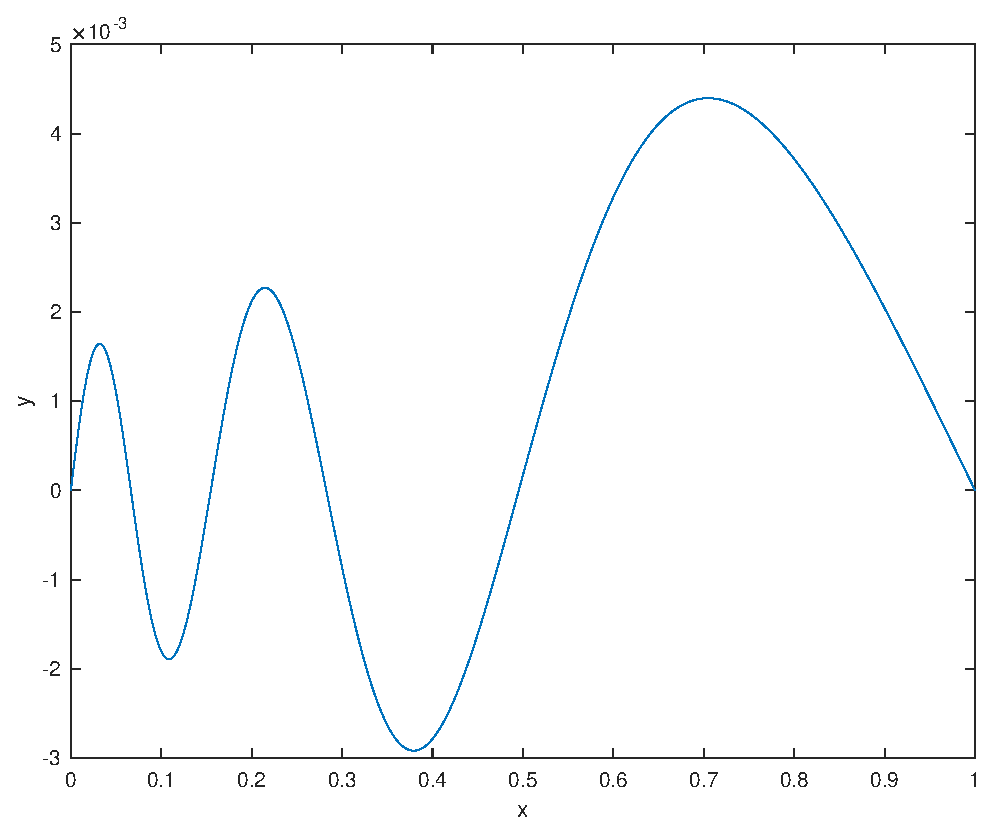
\includegraphics [width=4in]{Question_9_1_05.eps}



\end{document}
    
